%!TEX encoding = UTF-8 Unicode
% !TeX spellcheck = en_GB
%%%%%%%%%%%%%%%%%%%%%%%%%%%%%%%%%%%%%%
\chapter{Higgs and effective field theories }\label{chap:HiggsEFT}
%%%%%%%%%%%%%%%%%%%%%%%%%%%%%%%%%%%%%%
\par The study of the Higgs properties, couplings and rates aims to shed light on the structure of its potential and how and why it is responsible for the EW symmetry breaking. Explaining the vacuum expectation value and the mass of the Higgs has been the aim of many theoreticians and phenomenologists. This is because the SM provides no insights into the nature of the Higgs potential and its parameters.  In the SM, these input parameters need to be supplied from experimental observations. The Higgs potential shown in eq.~\eqref{higgspot} is the minimal one that could cause the EW symmetry breaking, but nature may not have taken this minimalist approach. 
\par  In order to test whether the Higgs potential is in the minimalist SM form or there are other more complex structures involved. One can start by measuring Higgs rates and confronting them against the SM prediction as overviewed in the previous chapter, using the $\kappa$ formalism.  Alas, this approach does not help understand what the new physics~(NP) structures would be more likely to cause a particular deviation. Conversely, we are interested in knowing what are the allowed NP structures given the current (or future) measurements of the Higgs rates.  Of course, by looking at concrete models, one would get insight into the aforementioned questions by confronting them with Higgs data. However, this is a  tedious task, as there are numerous ways NP might manifest~. 
\par In order to make the search for NP more accessible and model-agnostic, we could revert to~\textbf{effective field theories}~(EFT), one of the most perspicacious concepts of quantum field theory. In the EFT framework, the interactions mediated by  NP at the small scale of arbitrary complexity can be systematically simplified by approximating these interactions via integrating the UV degrees of freedom, leaving only numerable operators added to the SM. The premise of EFTs can be simply illustrated in~\autoref{fig:eft}.  For example, the LHC might not be able to resolve the UV degrees of freedom at their scale~$\Lambda$; rather, one can only observe the effective interactions they mediate. These new interactions depend on a set of free parameters known as~\textbf{Wilson coefficients}, which would be constrained or set from experiments. 
\begin{figure}[h!]
	\begin{center}
		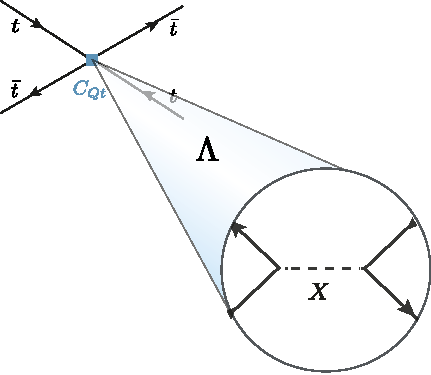
\includegraphics[width=.4 \linewidth]{figures/EFT}
		\caption{The premise of EFT stems from observing interactions at collider energy reach without being able to resolve the details of the NP mediating them, as the NP degrees of freedom have an energy scale $\Lambda$ higher than the collider's reach. }
		\label{fig:eft}
	\end{center}
\end{figure}
These ``phenomenological Lagrangians'' as called by Weinberg~\cite{WEINBERG1979327}, are not necessarily renormalisable but still allow for robust predictions that can be tested at colliders, including higher-order effects. \\
This chapter is organised as follows:  In ~\autoref{sec:smeft} the Higgs sector of Standard Model effective field theory~(SMEFT) will be presented along with the parametrisation of single and di-Higgs rates in terms of the SMEFT Wilson coefficients. In contrast to the SMEFT formalism, \autoref{sec:chiral} will present a non-linear EFT formalism known as the Chiral Lagrangian~(EWChL) or (Higgs)EFT. Finally, I will conclude this chapter with~\autoref{sec:concefts}.
%%%%%%%%%
\section{ The Standard Model effective field theory \label{sec:smeft}}
\par There is no unique way of defining an EFT for the Higgs boson~$h$. One could consider the field $h$ as an EW singlet or as a part of the doublet~$\phi$ like the SM. The first ansatz is more compatible with a heaver Higgs, and the effective coupling based on it could be derived from the EWChL as we shall see in~\autoref{sec:chiral}. However, after discovering the Higgs has a mass close to $m_Z$, the second option for an EFT seemed more fitting, though more restrictive. Assuming that the NP resonances would occur at masses $\Lambda \gg m_Z$, one can integrate them out, yielding a set of effective operators of mass dimension $> 4$.  Hence, one can think of the SM Lagrangian of mass dimensions $2$ and $4$ as a part of a more general EFT that contains the same fields and symmetries, known as the Standard Model Effective field theory~(SMEFT). 
\par From simple dimensional analysis, we know that the Higher dimensional operators need to contain an inverse mass with some power $p=4-d$ in the couplings, we have a clear power counting in the SMEFT Lagrangian, such that we could collect all operators of the same mass dimension~$d$ into a $d$-mass-dimensional Lagrangians taking the form
\begin{equation}
	\mathcal{L}^{(d)} = \frac{1}{\Lambda^{d-4}} \sum_i  C_i \mathcal{O}_i .
	\label{smeftdim}
\end{equation}
For any $d >4$, the Lagrangian in eq.~\eqref{smeftdim}  is not renormalisable in the strict sense, yet it is still predictive via fitting the Wilson coefficients~$C_i$ order-by-order to experimental measurements. This power-counting property allows for predictability even when we, in principle, have an infinite number of free Wilson coefficients, as all of these operators are suppressed by the NP scale~(irrelevant operators w.r.t. the renormalisation group). To illustrate this,  we let $\Lambda =1$, then the effects of dimension-six operators will be at the per cent level. At the same time, dimension-eight operators will have effects of order~$\sim10^{-4}$, allowing us to ignore the dimension-eight and higher operators.  Regarding dimension-five, we have only one operator called the Weinberg operator~\cite{PhysRevLett.43.1566}
\begin{equation}
	\mathcal{O}_{\nu \nu} =(\tilde{\phi} L_p)^T {\cal C} (\tilde{\phi}^{\dagger} L_q),
	\label{weinbergoperator}
\end{equation}
was $ \mathcal{C}$ is the charge conjugation operator. The Weinberg operator violates leptonic number and generates neutrino masses after EW symmetry breaking; similar effects are generated from dimension-seven operators~\cite{Lehman:2014jma}. These effects do not yield considerable collider phenomenology. Hence, I shall be discussing SMEFT with dimension-six operators only, for studies on Higher-dimensional SMEFT operators cf.~\cite{Lehman:2014jma,Lehman:2015coa,Henning:2015alf,Aguilar-Saavedra:2010uur}. \\ The SMEFT Lagrangian up to dimension-six operators is given by
%%%%%%%%%%
\begin{equation}
	\mathcal{L}_{\mathrm{SMEFT}}^{d=6}=\mathcal{L}_{\SM} + \frac{1}{\Lambda^2}\sum_i C_i  {\cal O}_i.
	\label{smeftdim6}
\end{equation}
%%%%%%%%%%%
\begin{table}
	\begin{center}
		\footnotesize
			\vspace{-.35cm}
		\hspace{-2.7 cm}
		\begin{minipage}[t]{4.6cm}
			\renewcommand{\arraystretch}{1.5}
			\begin{tabular}[t]{c|c}
				\multicolumn{2}{c}{$X^3$} \\
				\toplinetwo
				$\mathcal{O}_G$                & $f^{ABC} G_\mu^{A\nu} G_\nu^{B\rho} G_\rho^{C\mu} $ \\
				%
				$\mathcal{O}_{\widetilde G}$          & $f^{ABC} \widetilde G_\mu^{A\nu} G_\nu^{B\rho} G_\rho^{C\mu} $ \\
				%
				$\mathcal{O}_W$                & $\epsilon^{IJK} W_\mu^{I\nu} W_\nu^{J\rho} W_\rho^{K\mu}$ \\ 
				%
				$\mathcal{O}_{\widetilde W}$          & $\epsilon^{IJK} \widetilde W_\mu^{I\nu} W_\nu^{J\rho} W_\rho^{K\mu}$ \\
			\end{tabular}
		\end{minipage}
		%
		%
		%
		%
		\begin{minipage}[t]{4.6cm}
			\renewcommand{\arraystretch}{1.5}
			\begin{tabular}[t]{c|c}
				\multicolumn{2}{c}{Pure Higgs} \\
				\toplinetwo
				$\mathcal{O}_{\phi\Box}$ & $(\phi^\dag \phi)\Box(\phi^\dag \phi)$ \\
				%
				$\mathcal{O}_{\phi D}$   & $\ \left(\phi^\dag D_\mu \phi\right)^* \left(\phi^\dag D_\mu \phi\right)$ \\
				%
				$\mathcal{O}_\phi$       & $(\phi^\dag \phi)^3$ 
			\end{tabular}
		\end{minipage}
		%
		%
		\begin{minipage}[t]{2.7cm}
			
			\renewcommand{\arraystretch}{1.5}
			\begin{tabular}[t]{c|c}
				\multicolumn{2}{c}{$ \psi^2\phi^3 + \hbox{h.c.}$} \\
				\toplinetwo
				$\mathcal{O}_{e\phi}$           & $(\phi^\dag \phi)(\bar l_p e_r \phi)$ \\
				%
				$\mathcal{O}_{u\phi}$          & $(\phi^\dag \phi)(\bar q_p u_r \widetilde \phi )$ \\
				%
				$\mathcal{O}_{d\phi}$           & $(\phi^\dag \phi)(\bar q_p d_r \phi)$\\
			\end{tabular}
		\end{minipage}
		
		\vspace{0.25cm}
				\hspace{-2.7 cm}
		\begin{minipage}[t]{4.6cm}
			\renewcommand{\arraystretch}{1.5}
			\begin{tabular}[t]{c|c}
				\multicolumn{2}{c}{$X^2\phi^2$} \\
				\toplinetwo
				$\mathcal{O}_{\phi G}$     & $\phi^\dag \phi\, G^A_{\mu\nu} G^{A\mu\nu}$ \\
				%
				$\mathcal{O}_{\phi\widetilde G}$         & $\phi^\dag \phi\, \widetilde G^A_{\mu\nu} G^{A\mu\nu}$ \\
				%
				$\mathcal{O}_{\phi W}$     & $\phi^\dag \phi\, W^I_{\mu\nu} W^{I\mu\nu}$ \\
				%
				$\mathcal{O}_{\phi\widetilde W}$         & $\phi^\dag \phi\, \widetilde W^I_{\mu\nu} W^{I\mu\nu}$ \\
				%
				$\mathcal{O}_{\phi B}$     & $ \phi^\dag \phi\, B_{\mu\nu} B^{\mu\nu}$ \\
				%
				$\mathcal{O}_{\phi\widetilde B}$         & $\phi^\dag \phi\, \widetilde B_{\mu\nu} B^{\mu\nu}$ \\
				%
				$\mathcal{O}_{\phi WB}$     & $ \phi^\dag \tau^I \phi\, W^I_{\mu\nu} B^{\mu\nu}$ \\
				%
				$\mathcal{O}_{\phi\widetilde W B}$         & $\phi^\dag \tau^I \phi\, \widetilde W^I_{\mu\nu} B^{\mu\nu}$ 
			\end{tabular}
		\end{minipage}
		%
		%
		\begin{minipage}[t]{4.6cm}
			\renewcommand{\arraystretch}{1.5}
			\begin{tabular}[t]{c|c}
				\multicolumn{2}{c}{$\psi^2 X\phi+\hbox{h.c.}$} \\
				\toplinetwo
				$\mathcal{O}_{eW}$      & $(\bar l_p \sigma^{\mu\nu} e_r) \tau^I \phi W_{\mu\nu}^I$ \\
				%
				$\mathcal{O}_{eB}$        & $(\bar l_p \sigma^{\mu\nu} e_r) \phi B_{\mu\nu}$ \\
				%
				$\mathcal{O}_{uG}$        & $(\bar q_p \sigma^{\mu\nu} T^A u_r) \widetilde \phi \, G_{\mu\nu}^A$ \\
				%
				$\mathcal{O}_{uW}$        & $(\bar q_p \sigma^{\mu\nu} u_r) \tau^I \widetilde \phi \, W_{\mu\nu}^I$ \\
				%
				$\mathcal{O}_{uB}$        & $(\bar q_p \sigma^{\mu\nu} u_r) \widetilde \phi \, B_{\mu\nu}$ \\
				%
				$\mathcal{O}_{dG}$        & $(\bar q_p \sigma^{\mu\nu} T^A d_r) \phi\, G_{\mu\nu}^A$ \\
				%
				$\mathcal{O}_{dW}$         & $(\bar q_p \sigma^{\mu\nu} d_r) \tau^I \phi\, W_{\mu\nu}^I$ \\
				%
				$\mathcal{O}_{dB}$        & $(\bar q_p \sigma^{\mu\nu} d_r) \phi\, B_{\mu\nu}$ 
			\end{tabular}
		\end{minipage}
		%
		%
		\begin{minipage}[t]{2.7cm}
			\renewcommand{\arraystretch}{1.5}
			\begin{tabular}[t]{c|c}
				\multicolumn{2}{c}{$\psi^2\phi^2 D$} \\
				\toplinetwo
				$\mathcal{O}_{\phi l}^{(1)}$      & $(\phi^\dag i\overleftrightarrow{D}_\mu \phi)(\bar l_p \gamma^\mu l_r)$\\
				%
				$\mathcal{O}_{\phi l}^{(3)}$      & $(\phi^\dag i\overleftrightarrow{D}^I_\mu \phi)(\bar l_p \tau^I \gamma^\mu l_r)$\\
				%
				$\mathcal{O}_{\phi e}$            & $(\phi^\dag i\overleftrightarrow{D}_\mu \phi)(\bar e_p \gamma^\mu e_r)$\\
				%
				$\mathcal{O}_{\phi q}^{(1)}$      & $(\phi^\dag i\overleftrightarrow{D}_\mu \phi)(\bar q_p \gamma^\mu q_r)$\\
				%
				$\mathcal{O}_{\phi q}^{(3)}$      & $(\phi^\dag i\overleftrightarrow{D}^I_\mu \phi)(\bar q_p \tau^I \gamma^\mu q_r)$\\
				%
				$\mathcal{O}_{\phi u}$            & $(\phi^\dag i\overleftrightarrow{D}_\mu \phi)(\bar u_p \gamma^\mu u_r)$\\
				%
				$\mathcal{O}_{\phi d}$            & $(\phi^\dag i\overleftrightarrow{D}_\mu \phi)(\bar d_p \gamma^\mu d_r)$\\
				%
				$\mathcal{O}_{\phi u d}$ + h.c.   & $i(\widetilde \phi ^\dag D_\mu \phi)(\bar u_p \gamma^\mu d_r)$\\
			\end{tabular}
		\end{minipage}
		
		\vspace{0.25cm}
\hspace{-2.7 cm}
		
		\begin{minipage}[t]{4.95cm}
			\renewcommand{\arraystretch}{1.5}
			\begin{tabular}[t]{c|c}
				\multicolumn{2}{c}{$(\bar LL)(\bar LL)$} \\
				\toplinetwo
				$\mathcal{O}_{ll}$        & $(\bar l_p \gamma_\mu l_r)(\bar l_s \gamma^\mu l_t)$ \\
				%
				$\mathcal{O}_{qq}^{(1)}$  & $(\bar q_p \gamma_\mu q_r)(\bar q_s \gamma^\mu q_t)$ \\
				%
				$\mathcal{O}_{qq}^{(3)}$  & $(\bar q_p \gamma_\mu \tau^I q_r)(\bar q_s \gamma^\mu \tau^I q_t)$ \\
				%
				$\mathcal{O}_{lq}^{(1)}$                & $(\bar l_p \gamma_\mu l_r)(\bar q_s \gamma^\mu q_t)$ \\
				%
				$\mathcal{O}_{lq}^{(3)}$                & $(\bar l_p \gamma_\mu \tau^I l_r)(\bar q_s \gamma^\mu \tau^I q_t)$ 
			\end{tabular}
		\end{minipage}
		%
		%
		\begin{minipage}[t]{5.45cm}
			\renewcommand{\arraystretch}{1.5}
			\begin{tabular}[t]{c|c}
				\multicolumn{2}{c}{$(\bar RR)(\bar RR)$} \\
				\toplinetwo
				$\mathcal{O}_{ee}$               & $(\bar e_p \gamma_\mu e_r)(\bar e_s \gamma^\mu e_t)$ \\
				%
				$\mathcal{O}_{uu}$        & $(\bar u_p \gamma_\mu u_r)(\bar u_s \gamma^\mu u_t)$ \\
				%
				$\mathcal{O}_{dd}$        & $(\bar d_p \gamma_\mu d_r)(\bar d_s \gamma^\mu d_t)$ \\
				%
				$\mathcal{O}_{eu}$                      & $(\bar e_p \gamma_\mu e_r)(\bar u_s \gamma^\mu u_t)$ \\
				%
				$\mathcal{O}_{ed}$                      & $(\bar e_p \gamma_\mu e_r)(\bar d_s\gamma^\mu d_t)$ \\
				%
				$\mathcal{O}_{ud}^{(1)}$                & $(\bar u_p \gamma_\mu u_r)(\bar d_s \gamma^\mu d_t)$ \\
				%
				$\mathcal{O}_{ud}^{(8)}$                & $(\bar u_p \gamma_\mu T^A u_r)(\bar d_s \gamma^\mu T^A d_t)$ \\
				%
			\end{tabular}
		\end{minipage}

		\begin{minipage}[t]{4.95cm}
			\renewcommand{\arraystretch}{1.5}
			\begin{tabular}[t]{c|c}
				\multicolumn{2}{c}{$(\bar LL)(\bar RR)$} \\
				\toplinetwo
				$\mathcal{O}_{le}$               & $(\bar l_p \gamma_\mu l_r)(\bar e_s \gamma^\mu e_t)$ \\
				%
				$\mathcal{O}_{lu}$               & $(\bar l_p \gamma_\mu l_r)(\bar u_s \gamma^\mu u_t)$ \\
				%
				$\mathcal{O}_{ld}$               & $(\bar l_p \gamma_\mu l_r)(\bar d_s \gamma^\mu d_t)$ \\
				%
				$\mathcal{O}_{qe}$               & $(\bar q_p \gamma_\mu q_r)(\bar e_s \gamma^\mu e_t)$ \\
				%
				$\mathcal{O}_{qu}^{(1)}$         & $(\bar q_p \gamma_\mu q_r)(\bar u_s \gamma^\mu u_t)$ \\ 
				%
				$\mathcal{O}_{qu}^{(8)}$         & $(\bar q_p \gamma_\mu T^A q_r)(\bar u_s \gamma^\mu T^A u_t)$ \\ 
				%
				$\mathcal{O}_{qd}^{(1)}$ & $(\bar q_p \gamma_\mu q_r)(\bar d_s \gamma^\mu d_t)$ \\
				%
				$\mathcal{O}_{qd}^{(8)}$ & $(\bar q_p \gamma_\mu T^A q_r)(\bar d_s \gamma^\mu T^A d_t)$\\
			\end{tabular}
		\end{minipage}
		%
		%
		\begin{minipage}[t]{5.45 cm}
			\renewcommand{\arraystretch}{1.5}
			\begin{tabular}[t]{c|c}
				\multicolumn{2}{c}{$(\bar LR)(\bar L R)+\hbox{h.c.}$} \\
				\toplinetwo
				$\mathcal{O}_{quqd}^{(1)}$ & $(\bar q_p^j u_r) \epsilon_{jk} (\bar q_s^k d_t)$ \\
				%
				$\mathcal{O}_{quqd}^{(8)}$ & $(\bar q_p^j T^A u_r) \epsilon_{jk} (\bar q_s^k T^A d_t)$ \\
				%
				$\mathcal{O}_{lequ}^{(1)}$ & $(\bar l_p^j e_r) \epsilon_{jk} (\bar q_s^k u_t)$ \\
				%
				$\mathcal{O}_{lequ}^{(3)}$ & $(\bar l_p^j \sigma_{\mu\nu} e_r) \epsilon_{jk} (\bar q_s^k \sigma^{\mu\nu} u_t)$\\
				%
			 $\mathcal{O}_{ledq}$ & $(\bar l_p^j e_r)(\bar d_s q_{tj})$ 
			\end{tabular}
		\end{minipage}
	\end{center}
		\vspace{-.35cm}
	\caption{\label{warsaw}
	  Complete list of the dimension-six SMEFT operators in the Warsaw basis 
		\cite{Grzadkowski:2010es}. The $\mathcal{CP}$ violating operators contains the dual fields~$\widetilde X$. The flavour labels of the form $p,r,s,t$ on the $\mathcal{O}$ operators are suppressed on the left hand side of
		the tables.}
\end{table}
%%%%%%%%%%%
The study of dimension-six effective operators in characterising NP effects at energies beyond colliders’ reach has been first proposed in~\cite{BUCHMULLER1986621,Hagiwara:1993ck}. Nowadays,  phenomenological studies of EFTs with dimension-six operators primarily focus on using a set of complete and non-redundant ``basis''. This is since different effective operators will correspond to the same observables, e.g. same scattering amplitudes of SM particles.  This is the case if the operators can be related using equations of motion, Fierz transformations, integration by parts or field redefinitions. This leads to non-trivial and counter-intuitive relations between operators. Thus making the construction of the basis for the dimension-six SMEFT Lagrangian of eq.~\eqref{smeftdim6} a cumbersome task. Such task has been accomplished by~\cite{Grzadkowski:2010es} recently forming what is known as the \textbf{Warsaw Basis}.  Another set of basis is the strongly-interacting light Higgs basis (SILH), initially proposed by~\cite{Giudice:2007fh}, before the Warsaw basis and completed in ref.~\cite{Contino:2013kra, Elias-Miro:2013eta}. A more recent set of basis has been published in~\cite{Gupta:2014rxa} using a subset of couplings characterising the interactions of mass eigenstates in the effective Lagrangian.\\
The complete $d=6$ SMEFT is described by 2499 independent parameters~\cite{Jenkins:2013zjaJenkins:2013wua,Alonso:2013hga}. However, if one suppresses the flavour indices, assuming SMEFT is flavour blind, their inventory is significantly reduced. In the Warsaw basis, for example, assuming Baryon number conservation and dropping the flavour indices, one has only 59 operators, listed in~\autoref{warsaw}. It should be noted that all of the basis of SMEFT will produce the same phenomenology, though the choice of basis is sometimes helpful in simplifying the analysis. In this thesis, I will mainly focus on Warsaw basis.\\ 
The SMEFT operators can either modify SM parameters (couplings, masses) or introduce new vertices that do not exist in the SM, like four-fermion operators, or both like~$\mathcal{O}_{\phi e}$. An example of operators modifying SM parameters is $ \mathcal O_{\phi D}$, which leads to modification of the $Z$ boson mass after EW symmetry breaking 
\begin{equation}
	\frac{C_{\phi D}}{\Lambda^2} | \phi^\dagger D_\mu \phi |^2 \to \frac{C_{\phi D} v^4}{16 \Lambda^2 } (g_2^2+g_1^2) Z^\mu Z_\mu.
	\label{smeftdtoperatorim6}
\end{equation}
Additionally, from field redefinitions, we get indirect contributions to the $W$ mass from $C_{\phi D}$, combining both effects as a deviation in the $\rho$ parameter, we get
\begin{equation}
	\delta \rho = \frac{v^2}{2 \Lambda^2} C_{\phi D}.
	\label{rhosmeft}
\end{equation}
Which allows us to constrain $C_{\phi D}$ from the $T$ parameter 
\begin{equation}
	T = \frac{-2 \pi v^2}{\Lambda^2} \, \frac{(g_1^2 +g_2^2)}{g_1^2g_2^2} C_{\phi D}
	\label{smeftT}
\end{equation}
Another operator that affects the oblique parameters directly is $\mathcal{O}_{\phi W B}$, as it modifies the $S$ parameter in the following way
\begin{equation}
	S =\frac{16 \pi v^2}{g_1 g_2 \Lambda^2} C_{\phi W B}
	\label{smeftS}
\end{equation}
SM coupling modifications by SMEFT operators related to EWPO's are investigated in~\cite{Alasfar:2020mne}, and~\autoref{chap:flav}. Additionally, the contributions of the SMEFT Wilson coefficients to SM parameters are not only from tree-level effects like in eq.~\eqref{smeftdtoperatorim6} but could also come at loop-level, either from finite or RGE contributions.\\
SMEFT is suitable as a low energy limit for supersymmetric models~\cite{CARENA200363} or some classes of composite Higgs models~\cite{Contino:2010rs,Panico:2015jxa}
\subsection{Single Higgs processes in SMEFT}
Single Higgs production and decay processes are modified at LO by a relatively long list of operators summarised in~eqs.~\eqref{box:smefthiggslo}, ~\eqref{box:smefthiggslo2} and~\eqref{box:smefthiggslo3}. Explicit formulae for the Higgs rates dependence on the Wilson coefficients of these operators can be found in~\cite{ATLAS:2019dhi}
\begin{tcolorbox}[title=SMEFT operators modifying Higgs rates at LO,
	title filled=false,
	colback=Mahogany!5!white,
	colframe=Mahogany ]
	Higgs operators
	\begin{align}
		C_{\phi D}, \ \mathcal{O}_{\phi \Box},\ \mathcal{O}_{\phi G}, \ \mathcal{O}_{\phi W},\ \mathcal{O}_{\phi B}, \ \mathcal{O}_{\phi W B},\ \mathcal{O}_{\phi l}^{(1)}, \nn \\
		\ \mathcal{O}_{\phi l}^{(3)}, \ \mathcal{O}_{\phi e},\ \mathcal{O}_{\phi q}^{(1)},\ \mathcal{O}_{\phi q}^{(3)}, \  \mathcal{O}_{\phi u}, \ \mathcal{O}_{\phi d},\ \mathcal{O}_{\tau \phi}, \ \mathcal{O}_{t \phi}, \ \mathcal{O}_{b \phi},\ \mathcal{O}_{tb \phi}.
		\label{box:smefthiggslo}
	\end{align}
	Top-quark operators
	\begin{equation}
		\mathcal{O}_{t G}, \ \mathcal{O}_{t W}, \ \mathcal{O}_{t B},
		\label{box:smefthiggslo2}
	\end{equation}
	other 
	\begin{equation}
		\mathcal{O}_G,\ \mathcal{O}_{ll}^{(1)},\ \mathcal{O}_{Qq}^{(1),(3)},\ \mathcal{O}_{tu},\ \mathcal{O}_{td}^{(1),(8)},\ \mathcal{O}_{Qu}^{(1),(8)}, \ \mathcal{O}_{Qd}^{(1),(8)}.
		\label{box:smefthiggslo3}
	\end{equation}
	The third-generation quarks are denoted by~$Q$ while the first and second-generation quarks are assumed to have the same coupling and are denoted by $q,u,d$.
\end{tcolorbox}
Some of these operators are strongly constrained from EWPO data such as~$\mathcal{O}_{\phi D}$ and $ \mathcal{O}_{\phi W B}$, while others still have weak bounds from current measurements and are insensitive to EWPOs. Global fits on SMEFT Wilson coefficients can be found in ref.~\cite{Dawson:2020oco}, where Higgs and EW data were used to fit a subset of the SMEFT Wilson coefficients of the operators listed above. The fit also includes the effects of RGE and NLO (even NNLO for $m_W$). While in~\cite{Ethier:2021bye}, a global fit for a larger set of operators, but only with LO effects, including EW, Higgs and top data.  A more recent study~\cite{Dawson:2022bxd} has utilised EWPO data to constrain the four-fermion operators appearing in Higgs rates at LO and operators with four heavy quarks, using their NLO effects on EW bosons pole masses. We shall see in~\autoref{chap:4topSingleHiggs} that the latter operators also contribute to Higgs rates at NLO. A wider scope analysis including a wide range of Higgs, top, di-boson and EWPO data has been performed in~\cite{Ellis:2020unq}. \\
The dependence of single Higgs rates on the SMEFT Wilson coefficients gets more complicated once higher-order effects are taken into account. As shown in the fit results reported from~\cite{Dawson:2020oco}, the RGE of these Wilson coefficients introduces mixing with operators that do not appear at LO, also loop corrections to the rates and masses of the EW and Higgs bosons. \\A prominent example of an operator appearing only at NLO in single Higgs processes is $\mathcal O_\phi$, which modifies the Higgs self-interactions, namely the trilinear coupling. 
Typically, one ought to observe Higgs pair production to directly probe the Higgs trilinear self-coupling. However, due to the appearance of Higgs self-interaction and its modifiers, i.e.~$C_\phi$ in SMEFT context, in higher-order EW corrections~\cite{Degrassi:2014sxa,Kribs:2017znd} and Higgs observables~ \cite{McCullough:2013rea, Gorbahn:2016uoy, Degrassi:2016wml, Bizon:2016wgr, Maltoni:2017ims, Degrassi:2019yix, Degrassi:2021uik, Haisch:2021hvy}, one can extract bounds on the Higgs trilinear coupling from single Higgs and EWPO data. \autoref{fig:h_nlo_ew} illustrates example Feynman diagrams of single Higgs processes of which the trilinear Higgs self-coupling enters via NLO corrections.
\begin{figure}[htpb!]
	\begin{center}
		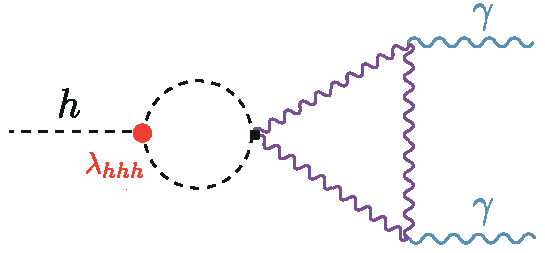
\includegraphics[width=0.8\textwidth]{figures/htoaa_nlo_ew}
		\caption{NLO EW corrections of single Higgs processes,  were the Higgs trilinear self-coupling~(the red circle) enters. Here the Higgs decay to two photons is shown as an example. \label{fig:h_nlo_ew} }
	\end{center}
\end{figure}
Using the results from the aforementioned references, a global fit with all operators that enter at tree-level in addition to the loop effects from the Higgs self-coupling has been preformed in refs.~\cite{DiVita:2017eyz,Dawson:2020oco}. Additionally, experimental searches for Higgs trilinear self-coupling have been presented by ATLAS~\cite{ATLAS:2019pbo} and CMS \cite{CMS:2020gsy}. 
%%%%%%%
\subsection{Higgs pair production and SMEFT}
Higgs pair production in hadron colliders is sensitive to six~$\mathcal{CP}$ even SMEFT operators \footnote{For or Higgs pair production with~$\mathcal{CP}$ violating operators, see ref.~\cite{Grober:2017gut}. }, under the assumption of Minimal Flavour violation~(MFV)~\footnote{MFV assumes that new physics operators will follow the same flavour hierarchies as the SM. }. These operators are
\begin{equation}
	\mathcal{O}_{\phi D},\ \mathcal{O}_{\phi \Box},\ \textcolor[HTML]{4334a0}{\mathcal{O}_{\phi}}, \ 	\textcolor[HTML]{2ebbaa}{\mathcal{O}_{t\phi}}, \ 	\textcolor[HTML]{ae0034}{\mathcal{O}_{\phi G}},\ \textcolor[HTML]{ffb743}{\mathcal{O}_{t G}},
	\label{HH-smeft}
\end{equation}
and their effects, with the corresponding colours are demonstrated in~\autoref{fig:hh-smeftw}, except for~$\mathcal{O}_{\phi D}$ and  $\mathcal{O}_{\phi \Box}$, as they modify all SM Higgs vertices. 
\begin{figure}[t!]
	\begin{center}
		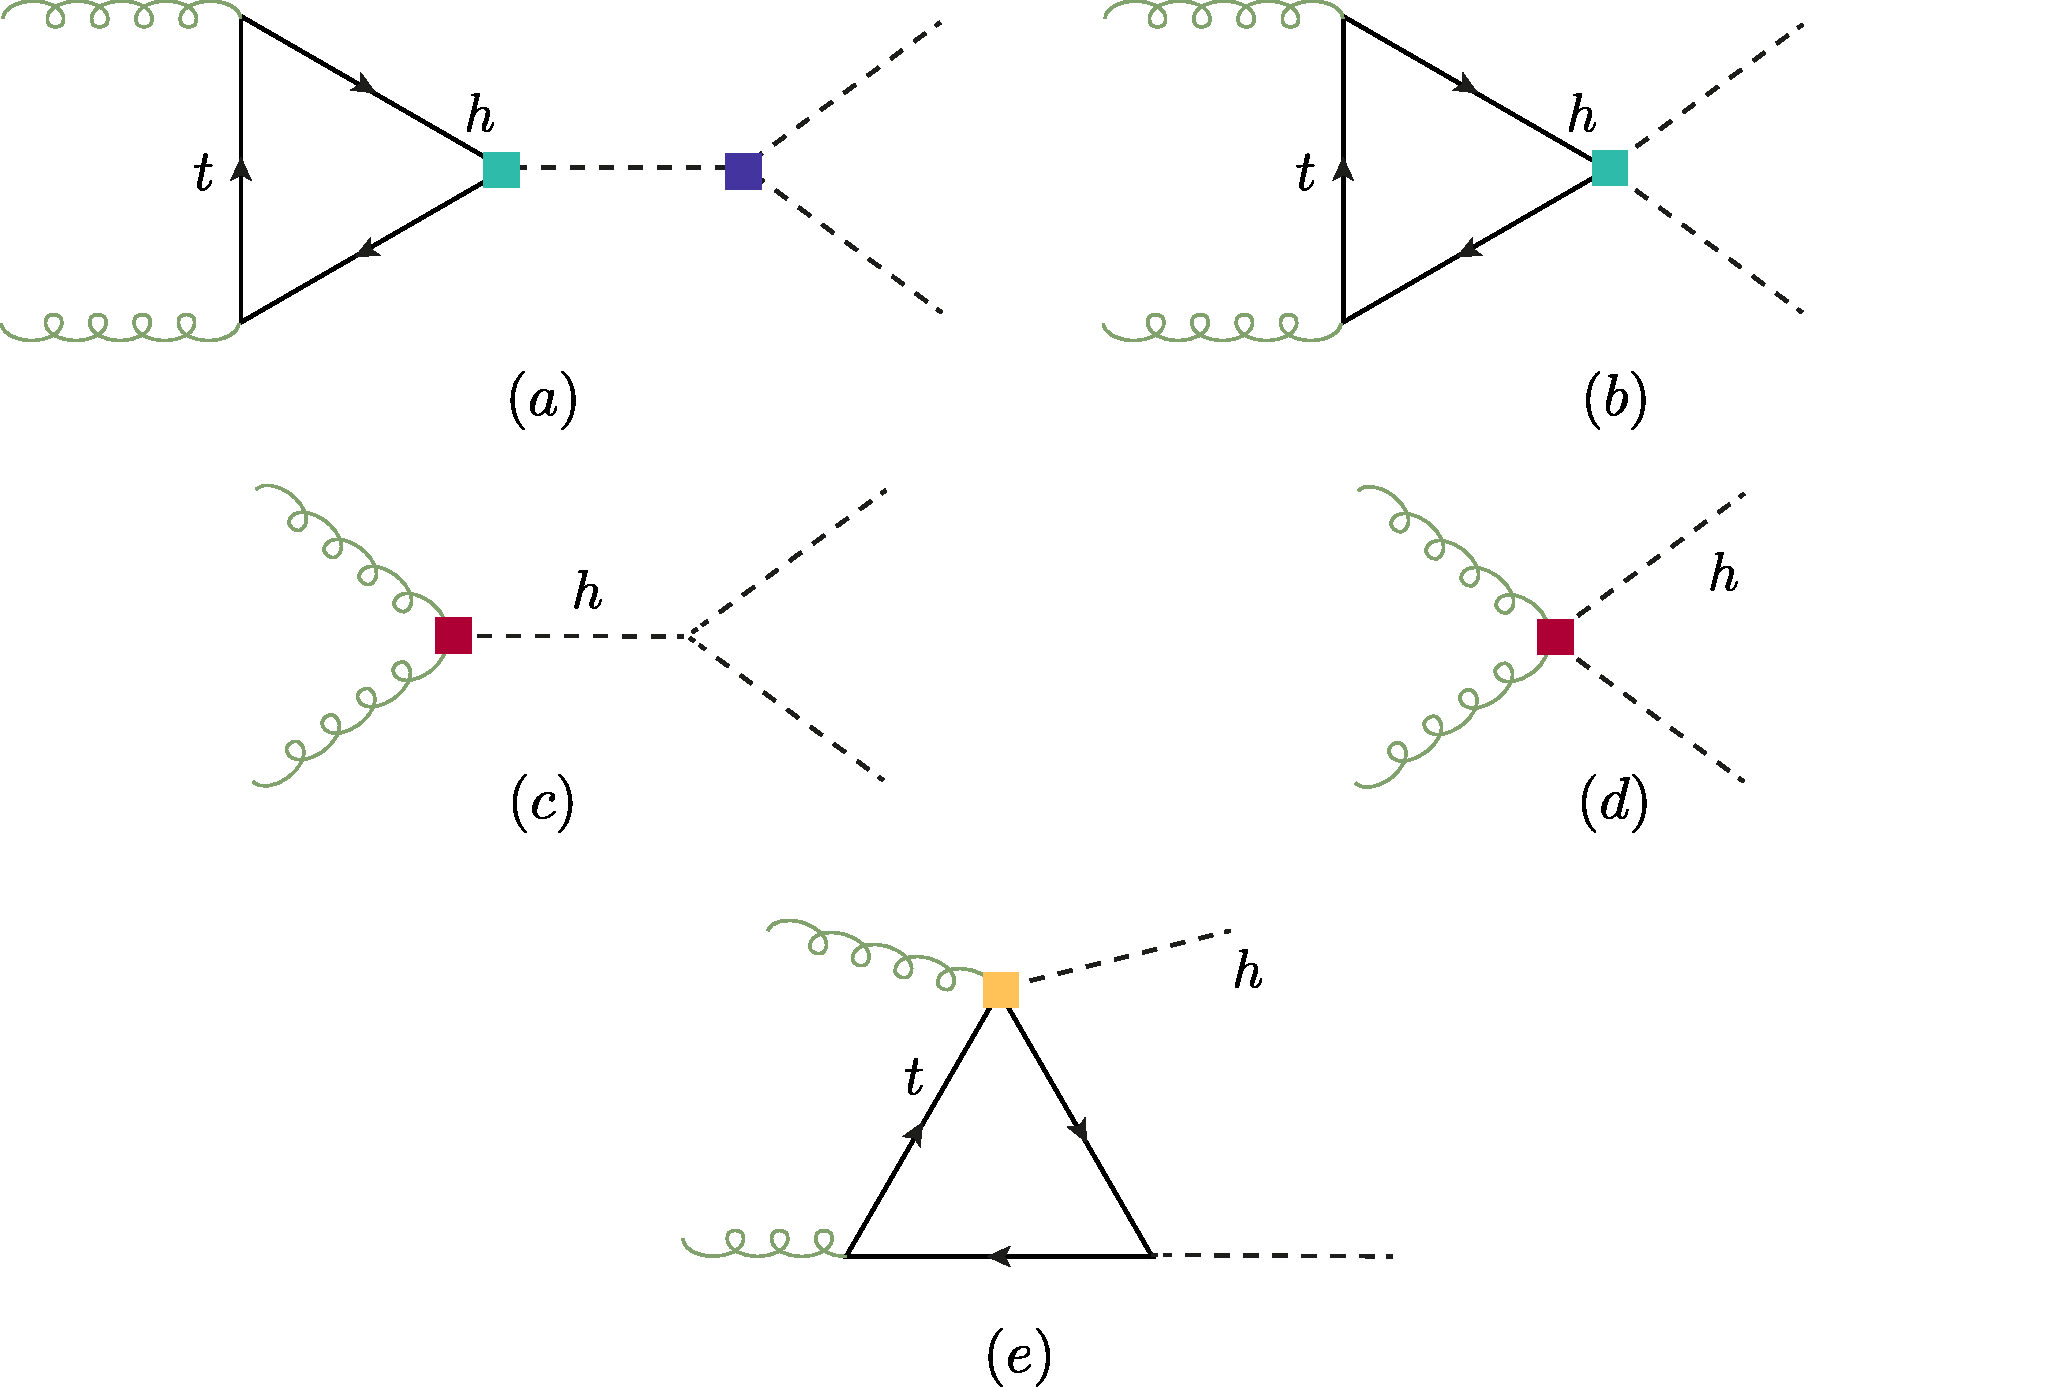
\includegraphics[width=0.75\textwidth]{figures/hh-smeft}
		\caption{ Example of diagrams illustrating how the dimension-six SMEFT operators enter in Higgs pair production at hadron colliders. \label{fig:hh-smeftw} }
	\end{center}
\end{figure}
However, MFV is not the only way to approach SMEFT, there exist more complex flavour structures that allow for significant enhancements of the first and second generation Yukawas without being excluded by flavour observables. Such formalisms will be discussed in~\autoref{chap:lightyuk}, in addition to  the potential for Higgs pair production in probing operators modifying light Yukawa couplings. 
The primary operator to constrain from Higgs pair as mentioned before is $\mathcal{O}_{\phi}$, for two reasons; a) the rest of the operators appearing tin di-Higgs are already strongly constrained from single Higgs and top processes. b) The effect of $\mathcal{O}_{\phi}$ on Higgs pair production is significantly higher than in single Higgs or EW observables. This is illustrated in~\autoref{fig:hh-vs-h} by comparing the relative change of the gluon fusion cross-sections at NLO QCD for single and di-Higgs production. This is not surprising since $C_\phi$ appears at LO in Higgs pair production.
\begin{figure}[h!]
	\begin{center}
		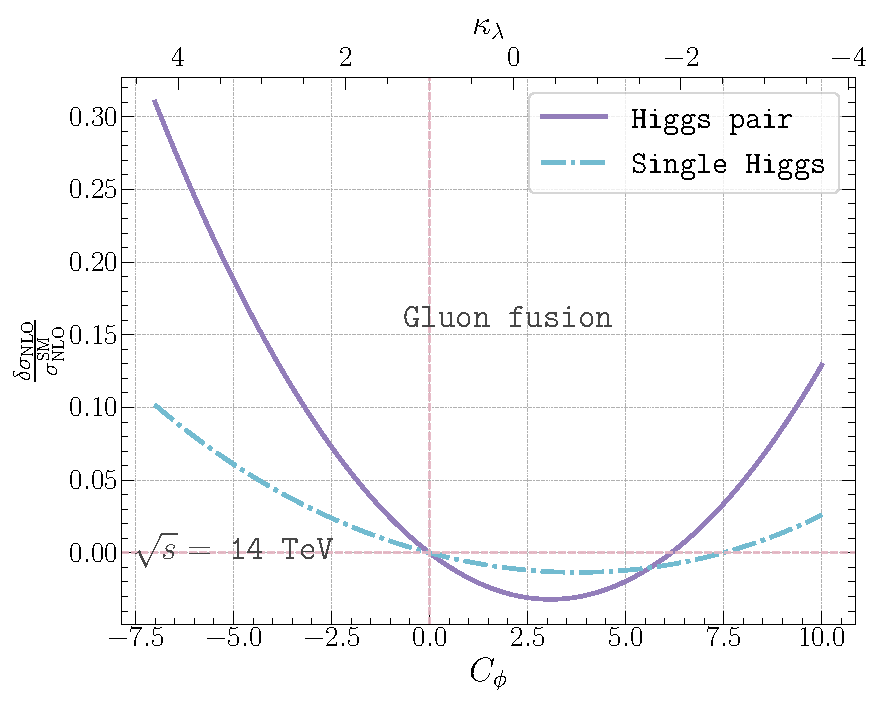
\includegraphics[width=0.65\textwidth]{figures/trilinear_single_vs_double}
		\caption{ The relative change of the NLO QCD cross-section of gluon fusion production of single Higgs (dashed line) and Higgs pair (solid line) at a $pp$ collider with $\sqrt{s}=14$ TeV as a function of $C_\phi$ or the corresponding $\kappa_\lambda$. \label{fig:hh-vs-h} }
	\end{center}
\end{figure}
Another advantage for Higgs pair production searches is the sensitivity of this process to non-linear couplings, for example, diagrams (b) and (d) of ~\autoref{fig:hh-smeftw}. Although in SMEFT, these diagrams correspond to the same operators in (a) and (c), respectively, in another EFT, this is not necessarily the case.
\section{The chiral Lagrangian \label{sec:chiral}}
Given the strong bonds on the $\rho$ parameter, it would be plausible to assume that the NP maintains the custodial symmetry~$SU(2)_V$and treats the chiral symmetry breaking pattern $SU(2)_L \otimes SU(2)_R \to SU(2)_V$  the same way the QCD chiral symmetry breaking is treated, in terms of considering the pions as pseudo-Nambu Goldstone bosons to describe their properties and couplings. In the pion case, this is known as \textbf{chiral perturbation theory}~\cite{GASSER1984142, GASSER1985465}. The same mathematical description could be applied to the case of EW symmetry breaking by constructing the EW chiral Lagrangian~(EWChL).   In this formalism, the Goldstone bosons~$\pi^a(x)$ of the SM are considered the generators of $SU(2)_L$ unitary transformation.
\begin{equation}
	\mathcal U(x) = e^{ i \pi^a(x)\sigma_a/v }, 
\end{equation}
which implies that the Goldstone fields transform non-linearly under~$SU(2)_L \otimes SU(2)_R$.  As for the Higgs boson~$h$, it is added as an $SU(2)_L \otimes U(1)_Y$ singlet, and can appear in the EWChL at any power. Contrary to the SMEFT power counting in the NP scale $ \Lambda$, in the EWChL, terms are ordered according to their \emph{chiral dimension} $\chi$, defined for spacetime derivatives $\partial_\mu$,  bosonic $\phi, X_\mu$ and $\psi$ fermionic generic fields as~\cite{Buchalla:2013rka,Buchalla:2015wfa}
\begin{equation}
	[\phi]_\chi =0,\,\, [X]_\chi =0,\,\, [\partial_\mu ]_\chi =1, \,\, [\psi]_\chi =2.
\end{equation}
The zeroth-order term of the EWChL possesses a chiral dimension of $\chi=2$, while higher-order terms could be considered terms generated perturbatively from $L$ loop interactions, with chiral dimension~$\chi= 2L+2$. The expansion of the EWChL is in the chiral order in addition to the powers of $h(x)/v$. This power-counting causes some SMEFT dimension-six operators to be considered of a higher order in HEFT. A prominent example of this is the chromomagnetic operator~$\mathcal O_{tG}$ being of chiral dimension 5 in EWChL. \\
The relevant terms for single- and di-Higgs production of the EWChL are given in the Unitary gauge by~\cite{LHCHiggsCrossSectionWorkingGroup:2016ypw,DiVita:2017eyz}
\begin{align}\nn
	\mathcal{L}_{\mathrm{HEFT}} = & \, \frac{h}{v} \Bigg[  \left( \delta c_W m_W^2 W_{\mu}^+W^{-\mu} +\delta c_Z \frac{m_Z^2}{2} Z_\mu Z^\mu\right)  \\\nn
	&+c_{ww}\frac{g_2^2}{2}W_{\mu\nu}^+W^{-\mu\nu} + c_{w\square} g_2^2\left(W_{\mu}^-\partial_\nu W^{+\mu\nu} + \text{h.c.}\right) +  c_{\gamma\gamma}\frac{\alpha}{8 \pi}A_{\mu\nu}A^{\mu\nu} \\\nn
	& +c_{zz}\frac{g_2^2 + g_1^2}{4} Z_{\mu\nu}Z^{\mu\nu}+ c_{z\gamma}\frac{e g_1}{16 \pi^2}Z_{\mu\nu}A^{\mu\nu}
	+c_{z\square}g_2^2Z_\mu\partial_\nu Z^{\mu\nu}
	+c_{\gamma \square}g_2 g_1 Z_\mu\partial_\nu A^{\mu\nu}
	\Bigg]\\\nn
	&+ \frac{\alpha_s}{8 \pi} \left( c_{gg} \frac{h}{v} +  c_{gg}^{(2)} \frac{h^2}{2 v^2}\right) \Tr[G_{\mu\nu} G^{\mu\nu}]
	-\sum_f \left[ m_f \left(c_f \frac{h}{v} + c _{ff} \frac{h^2}{2v^2}\right) \bar{f}_{R}f_{L}+\text{h.c.}\right]\\
	& - c_{hhh} \frac{m_h^2}{2 v} h^3\ + \dots,\label{eq:coupl_def}
\end{align}
I have omitted here the kinetic and mass terms of the Higgs, $\mathcal{CP}$ violating terms, as well as couplings not relearnt to LHC phenomenology and higher chiral order operators. \\
In addition to NP effects, this Lagrangian also includes the LO and NLO SM vertices, for example the parameter $\delta c_V=1$ corresponds to the tree-level coupling between the Higgs field and the EW bosons~$ V=W, Z$. While the coupling $c_{gg}= 4/3$ corresponds to the SM effective coupling at NLO if the heavy top limit~(HTL)~$m_t \to \infty$. \\
In contrast to the SMEFT, the couplings of one and two Higgs bosons to fermions or gluons become de-correlated. Giving this Lagrangian a richer phenomenology for Higgs pair production.  \\
The HEFT coefficients modifying the Higgs pair production via gluon fusion are 
\begin{equation}
	\textcolor[HTML]{4334a0}{c_{hhh} }, \ 	\textcolor[HTML]{2ebbaa}{c_t}\ (a) , \  	\textcolor[HTML]{2ebbaa}{c_{tt}} \ (b), \  \textcolor[HTML]{ae0034}{c_{gg}} \ (c), \  \textcolor[HTML]{ae0034}{c_{gg}^{(2)}} \ (d),
\end{equation}
with the same colours highlighted in the operator insertions of~\autoref{fig:hh-smeftw} and the letter next to the coefficient indicates the diagram, in which the coefficient appears .  Full parametrisation of the Higgs pair cross-section at NLO (inclusive and differential) and NNLO (inclusive)  can be found in refs.~\cite{Buchalla:2018yce,Capozi:2019xsi,deFlorian:2021azd} and implemented at NLO in \texttt{POWHEG-BOX}~\cite{Heinrich:2020ckp}. \\ UV-complete models that yield in the EWChL are composite Higgs models~\cite{Contino:2010rs,Panico:2015jxa,AGASHE2005165}, dilaton  theories~\cite{PhysRevLett.100.111802}, techni-dilaton models~\cite{Habaa:2010rbs}, technicolour models~\cite{Delgado:2010bb} and other models with induced EW symmetry breaking~\cite{Galloway:2013dma,Chang:2014ida}.
\subsection{Translation between SMEFT and HEFT }
In order to facilitate the translation between SMEFT and HEFT or to the $\kappa$-formalism, one needs to put the SMEFT Lagrangian into the canonical form, that is to convert the operators with covariant derivatives acting on the Higgs to  canonically normalised Higgs kinetic term. This is done done by the field redefinition.
\begin{equation}
	\phi=\left( \begin{array}{c} 0 \\ h(1+c_{h,kin}) + v \end{array} \right)
\end{equation} 
with 
\begin{equation}
	c_{h,kin}=\left(C_{\phi,\Box}-\frac{1}{4}C_{\phi D}\right) \frac{v^2}{\Lambda^2}\,.
\end{equation}
This field redefinition will generate derivative interactions of the form $h(\partial_{\mu}h)^2$ and $h^2(\partial_{\mu}h)^2$. In order to remove these terms, and for sake of simplicity, I use a gauge-dependent field redefinition\footnote{For gauge-independent formalism cf.~ \cite{Hartmann:2015aia}.}
\begin{equation}
	h \to h + c_{h,kin}\left( h +\frac{h^2}{v}+\frac{h^3}{3v^2}\right)\,. \label{fieldref}
\end{equation}
This field redefinition leads to n $c_{h,kin}$ modifying all Higgs couplings. \\
Before we discuss the translation between SMEFT and HEFT, some words of caution are in order: First, HEFT is less restrictive than SMEFT; therefore, it contains more degrees of freedom. This makes some points of the HEFT parameter space unmappable to SMEFT. In addition, the power counting is different in both formalisms. As mentioned before, some operators present in SMEFT will be absent in HEFT and vice-versa.  In ~\autoref{tab:translation}, the translation between the HEFT and SMEFT Wilson coefficients of the operators relevant to Higgs pair production at LO is shown. 
\begin{table}[htb]
	\begin{center}
		\begin{tabular}{ c c }
			\toplinetwo
			HEFT& SMEFT (Warsaw)\\
			\midrule
			$c_{hhh}$&$1-2\frac{v^4}{m_h^2}C_\phi+3c_{h,kin}$ \\
			$c_f$ & $1+c_{h,kin} -C_{f\phi} \frac{v^3}{\sqrt{2} m_f}$\\
			$ c_{ff} $ &$-C_{f\phi} \frac{3 v^3}{2\sqrt{2} m_f} + c_{h,kin}$\\
			$c_{gg}$  & $8\pi/\alpha_s v^2 C_{\phi G}$ \\
			$c_{gg}^{(2)}$  & $4\pi/\alpha_s v^2 C_{\phi G}$ \\
			\bottomrule
		\end{tabular}
	\end{center}
	\caption{Translation between the Wilson coefficients of HEFT and SMEFT for the operators relevant to Higgs pair production. \label{tab:translation}}
\end{table}
More general translation between SMEFT in Warsaw and SILH basis and HEFT can be done automatically using \texttt{Rosetta} package~\cite{Falkowski:2015wza}
\subsection{EFT and $\kappa$-formalism \label{eftkappa}}
The $\kappa$ formalism provides an experimentally accessible and well-defined QFT-wise approach to studying the Higgs properties. The $\kappa$ parameters are part of a more generalised formalism called the Higgs \textbf{Pseudo-observables}~\cite{Gonzalez-Alonso:2014eva} 
If the new physics contributions do not generate new Lorentz structures, there is a possible translation between the Wilson coefficients in the SMEFT Warsaw basis and the $\kappa$ formalism. In particular, taking the rescaling of the trilinear coupling, $\kappa_\lambda$, the translation is given by
\begin{equation}
	\kappa_\lambda = 1-\frac{2v^4}{m_h^2} \frac{C_\phi}{\Lambda^2}+3 c_{h,kin},
\end{equation}
A similar relation exists for the rescaling of the quark Yukawa couplings~$\kappa_q$
\begin{equation}
	\kappa_q = 1+c_{h,kin}- \frac{v^3}{\sqrt{2}m_q}\frac{C_{q\phi}}{\Lambda^2}.
\end{equation}
In these two examples, one can see the similarities between $\kappa$-formalism and HEFT, but this is not always the case.  Other translations could be obtained by comparing how SMEFT operators modify the Higgs couplings with the SM and matching it with the corresponding $\kappa$ or other Higgs pseudo-observable.\\ 
However, one should be careful while interpreting results quoted in terms of Wilson coefficients in the SMEFT framework extracted from multi-Higgs or multi-vector bosons searches. These results include couplings that are not present in the SM. For example, the $hh q\bar{q}$ coupling, though being linearly related to the quark Yukawa coupling $h q\bar{q}$, is not a rescaling of any SM Higgs coupling. With this in mind, one can strictly remain within a linear EFT and link the rescaling of the quark Yukawa, $\kappa_q$, to the~$hh q\bar{q}$ coupling through
\begin{equation}
	g_{hhq\bar{q}}^{\mathrm{linear-EFT}} = -\frac{3}{2}\frac{1-\kappa_q}{v} \, g_{h q\bar{q}}^{\mathrm{SM}}.
\end{equation}
This relation will no longer hold once a non-linear EFT, like HEFT, is used. Hence, the $\kappa$-formalism, in a strict sense, does not generally apply to multi-Higgs studies.
\section{Conclusions \label{sec:concefts}}
Effective field theories provide a systematic yet simplified approach for NP searches by simplifying its complex interaction structures. This can be viewed as a dimensionality reduction approach by collapsing all the NP interactions into effective ones. They would be observed at colliders with energy reaches below the NP scale $\Lambda$. The linear approach to EFT is called the SMEFT, which preserves the SM fields and symmetries, and the Higgs boson is a part of an $SU(2)_L$ doublet $\phi$ like the SM case. In contrast, non-linear approaches such as HEFT treat the Higgs boson as an added singlet. The latter approach is more general and introduces independent parameters involving multiple Higgs bosons. For example, the couplings $f\bar f h$ and $ f\bar f hh$ will be generated in SMEFT and HEFT. Still, in SMEFT, both are related by the Wilson coefficient $C_{\phi f}$, while in HEFT, they have independent  Wilson coefficients $c_f$ and $c_{ff}$, respectively. \\  Most of the Wilson coefficients involving Higgs interactions are strongly constrained by EWPOs and Higgs and top data. However, the bounds on the Wilson coefficient modifying Higgs self-couplings $C_\phi$ remain dominated by theoretical constraints from perturbative unitarity~\cite{DiLuzio:2017tfn,DiVita:2017vrr}. This can be improved by the searches for Higgs pair production at the HL-LHC, as this process is more sensitive to the trilinear Higgs self-coupling than EWPO and single-Higgs data.
%\begin{figure}[htbp!]
%	\begin{center}
	%		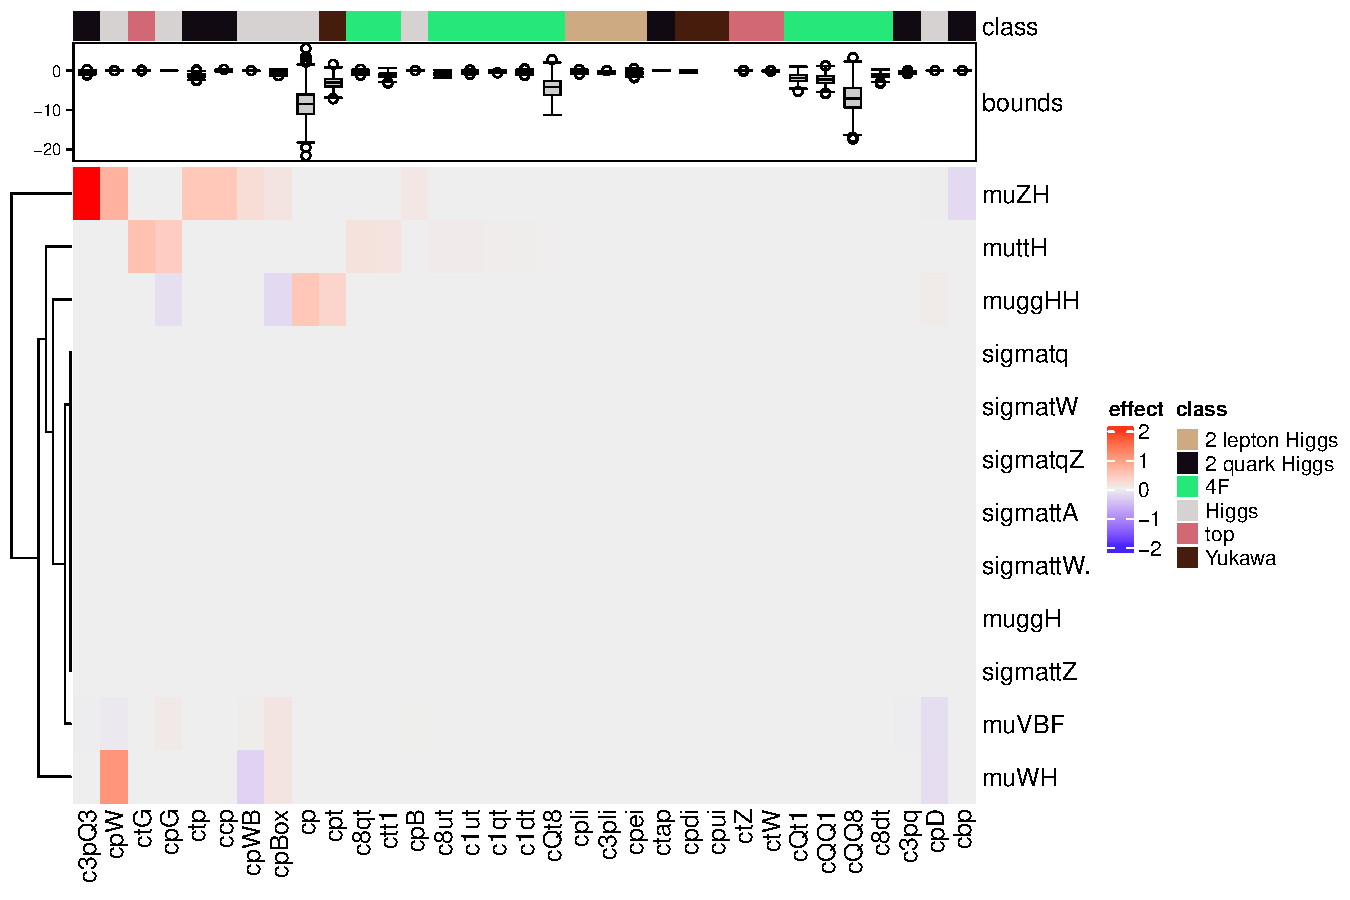
\includegraphics[width=\textwidth]{figures/smeft_heatmap}
	%		\caption{ \label{fig:greatheatmap} }
	%	\end{center}
%\end{figure}
%In~\autoref{greatheatmap}, I show the best bounds on the Wilson coefficients relearnt to Higgs production as well as heavy quark four-fermion operators, with a heatmap indicating the contribution of each operator in prominent Higgs, top and EW precision observables.  Although this is a subset of the total SMEFT operators and observables used in the fits, one can see the interconnectivity of the measurements.\\ The main objective of this thesis is to extend these connections by exploiting the potential of single-Higgs data and Higgs pair production to constrain the Higgs trilinear coupling modifiers (mainly in SMEFT) and the interplay between $C_\phi$ and heavy quark four-fermion operators in single Higgs data. Moreover, the SMEFT picture can be further extended by unravelling the interplay between Light quark couplings modifiers in Higgs pair production. Lastly, I will show another connection between Higgs operators in SMEFT and flavour anomalies.  Emphasising the complex interconnectivity between experimental observables and SMEFT operators. 
%%%%%%%
